\documentclass[10pt,letterpaper]{article}
\usepackage[margin=0.8in]{geometry}
\usepackage{amsmath,amssymb,graphicx,booktabs,xcolor,listings,fancyhdr}
\usepackage[colorlinks=true,linkcolor=blue!50!black,urlcolor=blue!50!black]{hyperref}
\setlength{\parindent}{0pt}
\setlength{\parskip}{5pt}
\setlength{\headheight}{14pt}
\pagestyle{fancy}
\fancyhf{}
\lhead{CSE276C \textbar\ Homework 1}
\rhead{Kinematics and Camera Calibration}
\cfoot{\thepage}
\newcommand{\R}{\mathbb{R}}
\newcommand{\T}{^{\mathsf T}}
\newcommand{\Afinal}{\begin{bmatrix}589.828760 & 0.000000 & 329.562979 \\ 0.000000 & 617.847616 & 267.857868 \\ 0.000000 & 0.000000 & 1.000000\end{bmatrix}}
\newcommand{\Afree}{\begin{bmatrix}606.149831 & 13.891421 & 340.393784 \\ 0.000000 & 610.282723 & 225.074278 \\ 0.000000 & 0.000000 & 1.000000\end{bmatrix}}
\newcommand{\bfinal}{\begin{bmatrix}1.916084\!\times\!10^{-6} \\ 0.000000 \\ -6.314704\!\times\!10^{-4} \\ 1.746239\!\times\!10^{-6} \\ -4.677439\!\times\!10^{-4} \\ 1.000000\!\times\!10^{0}\end{bmatrix}}
\newcommand{\bfree}{\begin{bmatrix}1.887510\!\times\!10^{-6} \\ -4.296401\!\times\!10^{-8} \\ -6.328265\!\times\!10^{-4} \\ 1.863009\!\times\!10^{-6} \\ -4.046908\!\times\!10^{-4} \\ 1.000000\!\times\!10^{0}\end{bmatrix}}
\lstset{language=Python,basicstyle=\ttfamily\footnotesize,
  keywordstyle=\color{blue!60!black},commentstyle=\color{green!35!black},
  stringstyle=\color{red!45!black},numbers=left,numberstyle=\tiny\color{gray},
  numbersep=8pt,breaklines=true,showstringspaces=false,columns=fullflexible,
  keepspaces=true,frame=single,rulecolor=\color{gray!35},tabsize=4}
\begin{document}
\begin{center}
{\LARGE\bfseries Homework 1}\\[5pt]
{\Large Kinematics and Camera Calibration}\\[5pt]
\textbf{Sachin Bhadang}\\
PID: A69040722\\
Email: \href{mailto:sbhadang@ucsd.edu}{sbhadang@ucsd.edu}\\[5pt]
CSE276C, Fall 2026 \hfill October 15, 2026
\end{center}

\section{Forward and inverse kinematics}
\subsection*{1(a): Reference frames and forward kinematics}
All lengths in this section are in centimeters. The world origin is the bottom
of the fixed base, with $+x$ right, $+y$ up, and $+z$ out of the page. The first
joint is at $(0,5)$. The three moving links each have length $\ell=10$.
Positive joint angles are counterclockwise about $+z$, measured relative to the
preceding link; all three angles are zero when the arm points along $+y$.
Consequently, negative angles bend a straight arm toward $+x$.

Put frame $J_i$ at joint $q_i$, with its $y_i$ axis along that joint's outgoing
link and its $x_i$ axis completing a right-handed frame. The absolute frame angles are
\[
\theta_0=q_0,\qquad \theta_1=q_0+q_1,\qquad
\theta_2=q_0+q_1+q_2.
\]
In a planar homogeneous representation, define
\[
\mathcal R(q)=\begin{bmatrix}\cos q&-\sin q&0\\
\sin q&\cos q&0\\0&0&1\end{bmatrix},\qquad
\mathcal D(d)=\begin{bmatrix}1&0&0\\0&1&d\\0&0&1\end{bmatrix}.
\]
The transform from the end-effector frame to the world frame is
\[
{}^WT_E=\mathcal D(5)\mathcal R(q_0)\mathcal D(10)
\mathcal R(q_1)\mathcal D(10)\mathcal R(q_2)\mathcal D(10).
\]
A link's displacement is its local vector $(0,10)\T$ rotated by its absolute
angle: $\mathcal R_{2\times2}(\theta)(0,10)\T
=10(-\sin\theta,\cos\theta)\T$. Adding these three displacements to the
fixed base offset gives
\begin{equation}
\boxed{\begin{aligned}
x(q)&=-10\,[\sin q_0+\sin(q_0+q_1)+\sin(q_0+q_1+q_2)],\\
y(q)&=5+10\,[\cos q_0+\cos(q_0+q_1)+\cos(q_0+q_1+q_2)].
\end{aligned}}
\end{equation}
As a check, $q=(0,0,0)\T$ gives $(x,y)=(0,35)$.

\subsection*{Differential motion model}
Differentiate the position with respect to the three joint angles. Writing
$c_i=\cos\theta_i$ and $s_i=\sin\theta_i$,
\begin{equation}
\boxed{\dot{\boldsymbol{x}}=T(q)\dot q,\qquad
T(q)=-10\begin{bmatrix}
c_0+c_1+c_2&c_1+c_2&c_2\\
s_0+s_1+s_2&s_1+s_2&s_2
\end{bmatrix}.}
\end{equation}
Angles in this derivative are in radians, so $T$ has units cm/rad and
$\dot{\boldsymbol{x}}$ has units cm/s when $\dot q$ is in rad/s.
At the straight pose, $T(0)=\left[\begin{smallmatrix}-30&-20&-10\\0&0&0\end{smallmatrix}\right]$,
which has rank one: instantaneous motion along the extended arm is unavailable.

\clearpage
\subsection*{1(b): A valid inverse-kinematics solution}
The desired displacement from the first joint is $(10,15)-(0,5)=(10,10)$.
Choose absolute link angles, measured counterclockwise from $+y$, symmetrically
about $-\pi/4$:
\[
(\theta_0,\theta_1,\theta_2)
=\left(\alpha-\frac\pi4,-\frac\pi4,-\alpha-\frac\pi4\right).
\]
For the unit direction $d(\theta)=(-\sin\theta,\cos\theta)\T$, the trigonometric
sum identities give
\[
d(-\pi/4+\alpha)+d(-\pi/4)+d(-\pi/4-\alpha)
=(1+2\cos\alpha)\frac{(1,1)\T}{\sqrt2}.
\]
Thus each component of the 10-cm-link sum equals 10 exactly if
\[
1+2\cos\alpha=\sqrt2,\qquad
\alpha=\arccos\left(\frac{\sqrt2-1}{2}\right)
=78.0471441093^\circ.
\]
Taking differences of consecutive absolute angles yields
\begin{equation}
\boxed{q=\begin{bmatrix}\alpha-\pi/4\\-\alpha\\-\alpha\end{bmatrix}
=\begin{bmatrix}33.0471441093^\circ\\-78.0471441093^\circ\\-78.0471441093^\circ\end{bmatrix}.}
\end{equation}
Every joint lies in $[-90^\circ,90^\circ]$. Substitution into the forward
kinematics gives $(x,y)=(10.000000,15.000000)$ cm, with numerical error
below $10^{-12}$ cm using the unrounded angles.

\begin{figure}[h!]
\centering
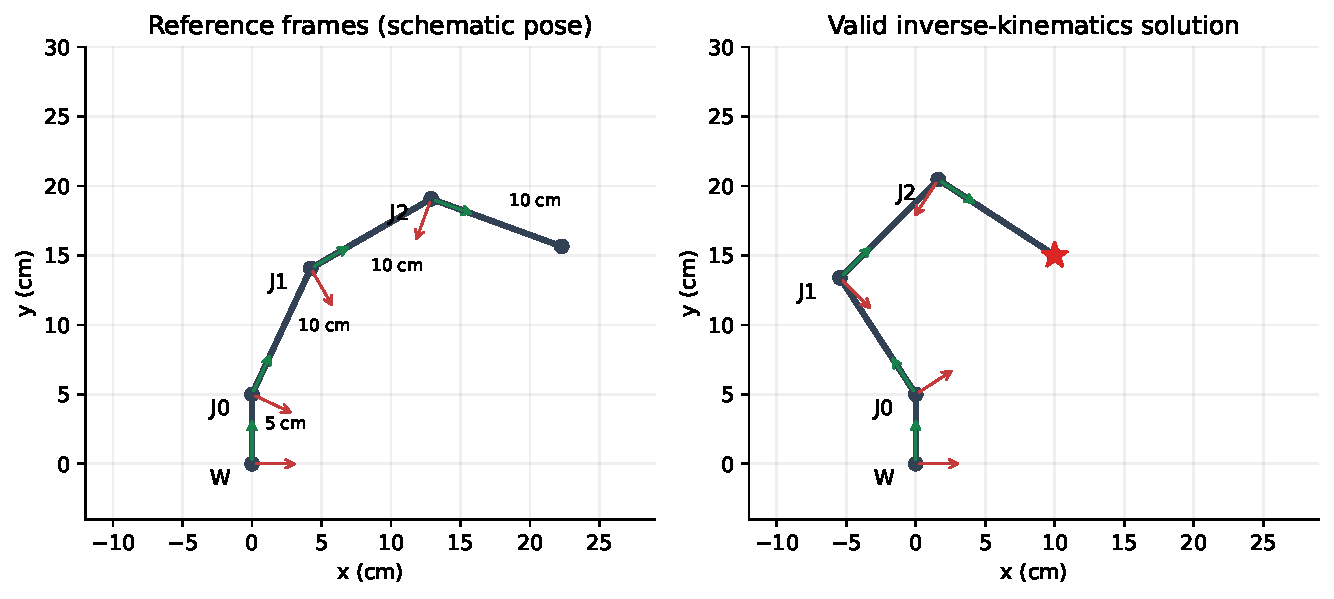
\includegraphics[width=\linewidth]{results/kinematics.pdf}
\caption{The assignment's arm geometry redrawn with world and joint frames
(left), and the computed IK configuration (right). Red arrows are local $+x$
axes; green arrows are local $+y$ axes; every $+z$ axis points out of the page.
$J_0,J_1,J_2$ are the frames at $q_0,q_1,q_2$. The star marks $(10,15)$ cm.}
\end{figure}

At this solution $T$ has rank two and a one-dimensional null space. A unit
null vector is
\[
n=\begin{bmatrix}0.4472135955&-0.6324555320&0.6324555320\end{bmatrix}\T,
\qquad Tn=0.
\]
Hence $\dot q=T^+\dot{\boldsymbol{x}}+\eta n$, with scalar $\eta$, realizes
the same instantaneous end-effector velocity. This explains the local
redundancy of the three-joint arm for a two-coordinate position task; the
closed-form construction above supplies the single solution requested.

\clearpage
\section{Camera calibration}
\subsection*{2.1(a): World coordinates and homography equations}
The input contains 432 pairs of pixel coordinates, grouped into nine
consecutive images with 48 points each. Within each image, eight points form
a left-to-right row and six rows run from top to bottom. With zero-based row
$r\in\{0,\ldots,5\}$ and column $c\in\{0,\ldots,7\}$, assign
\begin{equation}
P_{8r+c}=\begin{bmatrix}25c&25(5-r)&0\end{bmatrix}\T\ \text{mm},
\qquad p_{8r+c}=\begin{bmatrix}25c&25(5-r)&1\end{bmatrix}\T.
\end{equation}
The origin is the bottom-left \emph{detected corner}, not the outer paper
boundary. Thus the first file point has board coordinates $(0,125)$, point
7 has $(175,125)$, point 40 has $(0,0)$, and point 47 has $(175,0)$ mm.
World $X$ points right, $Y$ up the board, and $Z=X\times Y$.
Pixel $u$ increases rightward and $v$ downward. The detected-corner grid spans
$175\times125$ mm: eight corners define seven horizontal intervals and six
corners define five vertical intervals.

For $p_i=(X_i,Y_i,1)\T$ and $\tilde u_i=(u_i,v_i,1)\T$, the actual projective
relation is $s_i\tilde u_i=Hp_i$. Use the row-major vectorization
\[
h=(h_{11},h_{12},h_{13},h_{21},h_{22},h_{23},h_{31},h_{32},h_{33})\T.
\]
Eliminating $s_i=h_{31}X_i+h_{32}Y_i+h_{33}$ gives
\begin{align*}
h_{11}X_i+h_{12}Y_i+h_{13}-u_i(h_{31}X_i+h_{32}Y_i+h_{33})&=0,\\
h_{21}X_i+h_{22}Y_i+h_{23}-v_i(h_{31}X_i+h_{32}Y_i+h_{33})&=0.
\end{align*}
Therefore
\begin{equation}
\boxed{M_i=\begin{bmatrix}
X_i&Y_i&1&0&0&0&-u_iX_i&-u_iY_i&-u_i\\
0&0&0&X_i&Y_i&1&-v_iX_i&-v_iY_i&-v_i
\end{bmatrix},\qquad M_ih=0.}
\end{equation}
\begin{enumerate}
\item Each correspondence supplies \textbf{two independent scalar equations}.
\item $H$ has nine entries but is defined only up to nonzero scale, giving
\textbf{eight degrees of freedom}. Thus eight independent equations,
or \textbf{four correspondences in general position}, suffice. Collinear
or otherwise degenerate point arrangements do not suffice.
\item Each image supplies $2(48)=96$ equations for those eight degrees of
freedom. Its system is \textbf{overdetermined}, with $M\in\R^{96\times9}$.
\end{enumerate}

\subsection*{2.1(b): Homogeneous least squares}
For each view, stack its 48 blocks. The nonzero homogeneous least-squares
solution minimizes $\|Mh\|_2$ subject to $\|h\|_2=1$ and is the last right
singular vector of $M$. For numerical conditioning, both point sets are
first centered and scaled so their mean distance to the origin is $\sqrt2$.
If $p'=N_pp$ and $u'=N_uu$, solve for $H'$ in these coordinates and recover
\[
H=N_u^{-1}H'N_p,\qquad H\leftarrow H/H_{33}.
\]
This is a normalized linear DLT estimate, not a nonlinear minimization of
pixel error. All calculations use double precision. The nine matrices below
are rounded only for display; subsequent calculations use their full precision.

\clearpage
\subsection*{Homography matrices, in image-file order}
These matrices map board coordinates in millimeters to homogeneous image
coordinates, with $H_{33}=1$. Reprojection divides by the third coordinate.
\begingroup
\small
\setlength{\jot}{8pt}
\begin{align*}
H_{1} &= \begin{bmatrix}1.529753 & 0.495223 & 114.097565 \\ -0.098593 & -0.411171 & 273.823693 \\ 0.000188 & 0.001976 & 1.000000\end{bmatrix} \\
H_{2} &= \begin{bmatrix}1.628322 & 0.253506 & 196.146199 \\ -0.015484 & -0.433359 & 275.202229 \\ 0.000568 & 0.001905 & 1.000000\end{bmatrix} \\
H_{3} &= \begin{bmatrix}1.768884 & -0.057453 & 148.550326 \\ 0.041759 & -0.652196 & 323.144120 \\ 0.001084 & 0.001649 & 1.000000\end{bmatrix} \\
H_{4} &= \begin{bmatrix}1.974559 & -0.260418 & 269.206560 \\ 0.114267 & -0.810967 & 310.181257 \\ 0.001481 & 0.001672 & 1.000000\end{bmatrix} \\
H_{5} &= \begin{bmatrix}1.789825 & -0.232785 & 225.412112 \\ 0.110863 & -0.728106 & 381.443616 \\ 0.001374 & 0.001515 & 1.000000\end{bmatrix} \\
H_{6} &= \begin{bmatrix}1.782385 & -0.373168 & 248.937937 \\ 0.168182 & -0.771653 & 337.649892 \\ 0.001601 & 0.001374 & 1.000000\end{bmatrix} \\
H_{7} &= \begin{bmatrix}1.829844 & -0.379205 & 175.973039 \\ 0.185915 & -0.781881 & 392.693150 \\ 0.001697 & 0.001400 & 1.000000\end{bmatrix} \\
H_{8} &= \begin{bmatrix}1.725898 & -0.385103 & 325.095087 \\ -0.032442 & -0.829978 & 325.513611 \\ 0.001346 & 0.001273 & 1.000000\end{bmatrix} \\
H_{9} &= \begin{bmatrix}1.720368 & -0.279565 & 321.685119 \\ 0.142670 & -0.576736 & 322.016662 \\ 0.001403 & 0.001563 & 1.000000\end{bmatrix} \\
\end{align*}
\endgroup

\clearpage
\subsection*{Reprojection errors}
For every view $j$ and corner $i$, compute the Euclidean pixel error
\[
e_{ji}=\left\|\begin{bmatrix}u_{ji}\\v_{ji}\end{bmatrix}
-\pi(H_jp_i)\right\|_2,\qquad
\pi(a,b,c)=(a/c,b/c)\T.
\]
The requested total is $\boxed{\sum_{j,i}e_{ji}=162.931123\ \mathrm{pixels}}$.
Across all 432 corners, the mean is $0.377155$ pixels and the pointwise RMS
is $\sqrt{\sum e_{ji}^2/432}=0.434518$ pixels. For clarity, the sum of
\emph{squared} errors is a different quantity: $81.563984\ \mathrm{pixels}^2$.

\begin{center}
\small
\begin{tabular}{rrrrr}\toprule
View & Sum (px) & Mean (px) & RMS (px) & Maximum (px)\\\midrule
1 & 20.409515 & 0.425198 & 0.487243 & 0.934292 \\
2 & 18.998046 & 0.395793 & 0.456896 & 1.001749 \\
3 & 17.915610 & 0.373242 & 0.424739 & 0.912635 \\
4 & 20.019560 & 0.417074 & 0.474302 & 0.955674 \\
5 & 16.041796 & 0.334204 & 0.392116 & 0.869267 \\
6 & 17.357986 & 0.361625 & 0.417608 & 0.884603 \\
7 & 16.904627 & 0.352180 & 0.410637 & 0.832270 \\
8 & 16.594989 & 0.345729 & 0.396308 & 0.795087 \\
9 & 18.688993 & 0.389354 & 0.440330 & 0.894420 \\
\bottomrule\end{tabular}

\end{center}
\begin{figure}[h!]
\centering
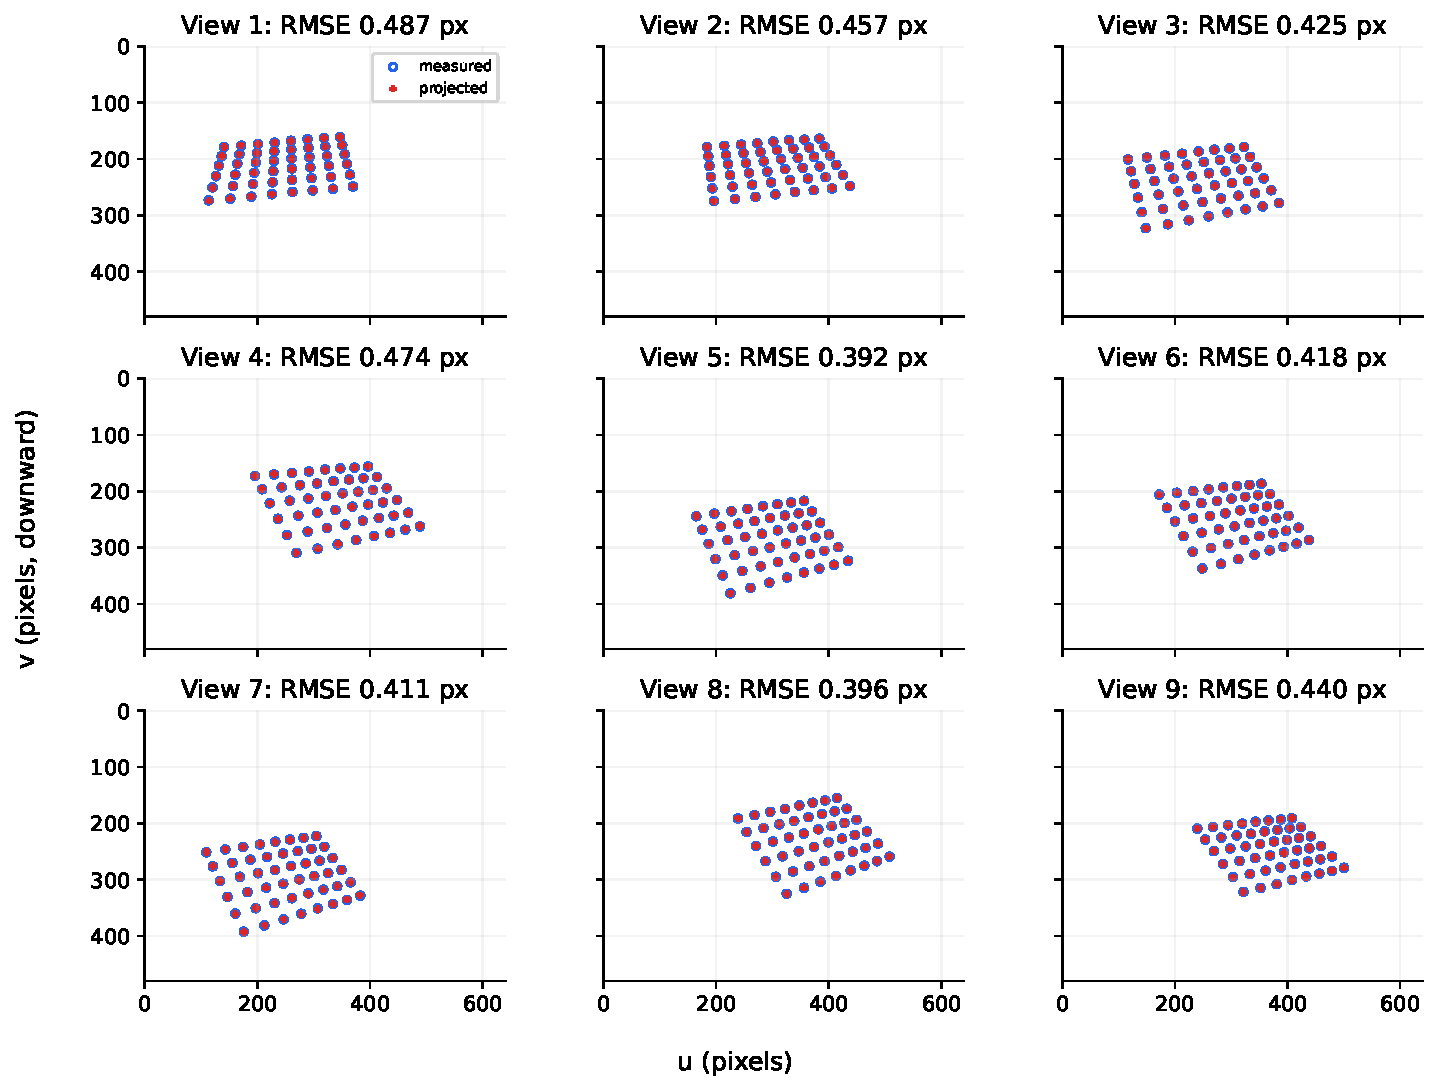
\includegraphics[width=0.88\linewidth]{results/reprojections.pdf}
\caption{Measured corners and normalized-DLT reprojections for all nine
views. The subpixel discrepancies are small at the scale of the full
$640\times480$ images.}
\end{figure}

\clearpage
\subsection*{2.2(a--b): Constraints on the intrinsic matrix}
Let $H=[h_1\ h_2\ h_3]$ and $B=A^{-\mathsf T}A^{-1}$. Use the
\emph{assignment's} vector order
\[
b=(b_{11},b_{12},b_{13},b_{22},b_{23},b_{33})\T,\qquad
B=\begin{bmatrix}b_{11}&b_{12}&b_{13}\\b_{12}&b_{22}&b_{23}\\
b_{13}&b_{23}&b_{33}\end{bmatrix}.
\]
For column vectors $h_i=(h_{1i},h_{2i},h_{3i})\T$, direct expansion gives
$h_i\T B h_j=v_{ij}\T b$, where
\[
v_{ij}=\begin{bmatrix}
h_{1i}h_{1j}\\h_{1i}h_{2j}+h_{2i}h_{1j}\\
h_{1i}h_{3j}+h_{3i}h_{1j}\\h_{2i}h_{2j}\\
h_{2i}h_{3j}+h_{3i}h_{2j}\\h_{3i}h_{3j}
\end{bmatrix}.
\]
The orthogonality and equal-length constraints therefore become
\begin{equation}
\boxed{L_jb=0,\qquad L_j=\begin{bmatrix}
v_{12}\T\\(v_{11}-v_{22})\T
\end{bmatrix},\qquad L=\begin{bmatrix}L_1\\\vdots\\L_9\end{bmatrix}.}
\end{equation}
\begin{enumerate}
\item Each homography supplies \textbf{two scalar constraints}.
\item A general symmetric $B$ has six entries, or five degrees of freedom
after scale is removed. Thus \textbf{three suitably different views} are
needed for the unconstrained six-vector solution. If zero skew is imposed,
$b_{12}=0$ removes another degree of freedom, and \textbf{two nondegenerate
views} can suffice. Merely translating a board at fixed orientation does
not supply the required diversity.
\item With nine views, $L$ is $18\times6$, so this is \textbf{overdetermined}
for either model.
\end{enumerate}
For the specified six-vector solve, the last right singular vector of $L$
gives $b_{\rm free}$. To also enforce the assignment's opening assumption of
no skew, remove the column multiplying $b_{12}$, solve the resulting
$18\times5$ system, and insert $b_{12}=0$ exactly. This gives $b_0$.
Both are normalized to $b_{33}=1$ below:
\[
\begin{aligned}
b_{\rm free}&=\bfree,&\qquad b_0&=\bfinal.
\end{aligned}
\]
Both reconstructed $B$ matrices are positive definite. The six singular
values of $L$ are approximately
\[
(9.27759,3.83942,0.473113,0.00611026,0.000445818,2.78357\times10^{-7}).
\]
Noise makes the smallest value nonzero; its right singular vector supplies
the least-squares solution.

\clearpage
\subsection*{2.2(c--d): Recovering and interpreting $A$}
With $d=b_{11}b_{22}-b_{12}^2$, the intrinsic recovery formulas are
\begin{align*}
c_y&=\frac{b_{12}b_{13}-b_{11}b_{23}}{d},&
\lambda_B&=b_{33}-\frac{b_{13}^2+c_y(b_{12}b_{13}-b_{11}b_{23})}{b_{11}},\\
f_x&=\sqrt{\lambda_B/b_{11}},&f_y&=\sqrt{\lambda_B b_{11}/d},\\
\gamma&=-\frac{b_{12}f_x^2f_y}{\lambda_B},&
c_x&=\frac{\gamma c_y}{f_y}-\frac{b_{13}f_x^2}{\lambda_B}.
\end{align*}
These follow the closed-form method and Appendix B of Zhang's
calibration report; its vector ordering differs from the one required here.
The general six-vector solution yields
\[
A_{\rm free}=\Afree.
\]
Its estimated skew is $13.891421$ pixels. To satisfy the stipulated
zero-skew model, the remaining calculations instead use the constrained fit
\begin{equation}
\boxed{A=A_0=\Afinal.}
\end{equation}
This is obtained by re-solving with $b_{12}=0$, not by changing just one
entry of $A_{\rm free}$ after fitting.

\begin{center}
\begin{tabular}{lll}
\toprule
Entry & Estimate & Meaning\\
\midrule
$A_{11}=f_x$ & $589.828760$ px & Horizontal focal scale\\
$A_{22}=f_y$ & $617.847616$ px & Vertical focal scale\\
$A_{13}=c_x$ & $329.562979$ px & Principal point, horizontal coordinate\\
$A_{23}=c_y$ & $267.857868$ px & Principal point, vertical coordinate\\
$A_{12}=\gamma$ & $0$ & Enforced zero skew\\
$A_{21},A_{31},A_{32}$ & $0$ & Canonical upper-triangular camera convention\\
$A_{33}$ & $1$ & Homogeneous normalization\\
\bottomrule
\end{tabular}
\end{center}
Relative to the nominal image center $(320,240)$, the principal point is
shifted by $(9.563,27.858)$ pixels. Using zero-based pixel-center coordinates
would place the geometric center at $(319.5,239.5)$ instead. The focal-scale
ratio is $f_x/f_y\approx0.954651$.

A centered camera with square pixels would suggest $c_x\approx320$,
$c_y\approx240$, and $f_x\approx f_y$. However, the ideal pinhole model
itself does \emph{not} require an exactly centered principal point or equal
focal scales: unequal pixel spacing or image resizing can produce unequal
$f_x,f_y$. Possible estimation discrepancies include corner localization
error, finite and similar viewing directions, checkerboard flatness or
printing error, unmodeled lens distortion, and sensor/lens misalignment.
The visible change between the constrained and unconstrained estimates is
evidence of sensitivity to the modeling constraint, not proof of physical
sensor skew. Ground-truth intrinsics are not supplied.

Only the linear calibration steps requested are used; no lens-distortion
parameters or nonlinear refinement are fitted.

\clearpage
\subsection*{2.3(a): Extrinsic recovery}
For each $H$, compute $Q=A^{-1}H=[a_1\ a_2\ a_3]$. Ideally the first two
columns have equal norms. With noisy estimates, use their symmetric scale
\[
\rho=\frac{2}{\|a_1\|+\|a_2\|},\qquad
\tilde r_1=\rho a_1,\quad \tilde r_2=\rho a_2,\quad
\tilde r_3=\tilde r_1\times\tilde r_2,\quad t=\rho a_3.
\]
Choose the sign of $\rho$ so the board origin has positive camera depth.
To enforce a proper rotation, take
$\tilde R=U\Sigma V\T$ and set
\[
R=U\operatorname{diag}(1,1,\det(UV\T))V\T.
\]
This applies the Section 3.1 pose construction and Appendix C rotation
projection of Zhang's report, with a determinant correction to ensure $\det R=+1$.
All matrices below map \emph{world to camera}:
$X_c=RX_w+t$. Translations are in millimeters; $R$ is dimensionless.
\begingroup
\small
\setlength{\jot}{6pt}
\begin{align*}
[R_{1}\mid t_{1}] &= \begin{bmatrix}0.99328 & -0.11174 & -0.03027 & -145.66812 \\ -0.09227 & -0.60628 & -0.78988 & 3.85037 \\ 0.06991 & 0.78736 & -0.61252 & 398.76120\end{bmatrix} \\
[R_{2}\mid t_{2}] &= \begin{bmatrix}0.96735 & -0.24739 & 0.05504 & -89.64586 \\ -0.11011 & -0.60584 & -0.78793 & 4.71106 \\ 0.22827 & 0.75615 & -0.61330 & 396.31976\end{bmatrix} \\
[R_{3}\mid t_{3}] &= \begin{bmatrix}0.90219 & -0.39205 & 0.17989 & -116.16425 \\ -0.14842 & -0.67372 & -0.72393 & 33.87079 \\ 0.40501 & 0.62642 & -0.66600 & 378.52060\end{bmatrix} \\
[R_{4}\mid t_{4}] &= \begin{bmatrix}0.85029 & -0.45981 & 0.25608 & -34.50038 \\ -0.15682 & -0.68580 & -0.71069 & 23.09540 \\ 0.50240 & 0.56414 & -0.65524 & 337.15247\end{bmatrix} \\
[R_{5}\mid t_{5}] &= \begin{bmatrix}0.84583 & -0.46433 & 0.26262 & -65.80242 \\ -0.15361 & -0.68346 & -0.71364 & 68.50897 \\ 0.51086 & 0.56328 & -0.64942 & 372.65328\end{bmatrix} \\
\end{align*}
\begin{align*}
[R_{6}\mid t_{6}] &= \begin{bmatrix}0.78912 & -0.51999 & 0.32696 & -50.73176 \\ -0.15655 & -0.68498 & -0.71155 & 41.92377 \\ 0.59395 & 0.51031 & -0.62193 & 371.13839\end{bmatrix} \\
[R_{7}\mid t_{7}] &= \begin{bmatrix}0.78003 & -0.52666 & 0.33791 & -94.44216 \\ -0.15125 & -0.68269 & -0.71488 & 73.27993 \\ 0.60719 & 0.50651 & -0.61218 & 362.68456\end{bmatrix} \\
[R_{8}\mid t_{8}] &= \begin{bmatrix}0.82339 & -0.51020 & 0.24843 & -2.86115 \\ -0.24378 & -0.71335 & -0.65704 & 35.24724 \\ 0.51244 & 0.48044 & -0.71175 & 377.71473\end{bmatrix} \\
[R_{9}\mid t_{9}] &= \begin{bmatrix}0.82370 & -0.51025 & 0.24732 & -5.13871 \\ -0.14957 & -0.61623 & -0.77323 & 33.72559 \\ 0.54695 & 0.59992 & -0.58390 & 384.74411\end{bmatrix} \\
\end{align*}
\endgroup

\clearpage
\subsection*{2.3(b): Camera trajectory}
The world-coordinate camera center is the point that maps to zero in camera
coordinates. Thus
\[
RC+t=0\quad\Longrightarrow\quad\boxed{C=-R^{-1}t=-R\T t}.
\]
The resulting centers, relative to the bottom-left detected board corner, are
\begin{center}
\begin{tabular}{rrrr}\toprule
View & $C_X$ (mm) & $C_Y$ (mm) & $C_Z$ (mm)\\\midrule
1 & 117.1667 & -327.9113 & 242.8800 \\
2 & -3.2290 & -318.9985 & 251.7091 \\
3 & -43.4764 & -259.8366 & 297.5130 \\
4 & -136.4297 & -190.2251 & 246.1642 \\
5 & -124.1907 & -193.6374 & 308.1804 \\
6 & -173.8430 & -187.0587 & 277.2412 \\
7 & -135.4673 & -183.4166 & 306.3272 \\
8 & -182.6076 & -157.7843 & 292.7073 \\
9 & -201.1592 & -212.6542 & 252.0020 \\
\bottomrule\end{tabular}

\end{center}
\begin{figure}[h!]
\centering
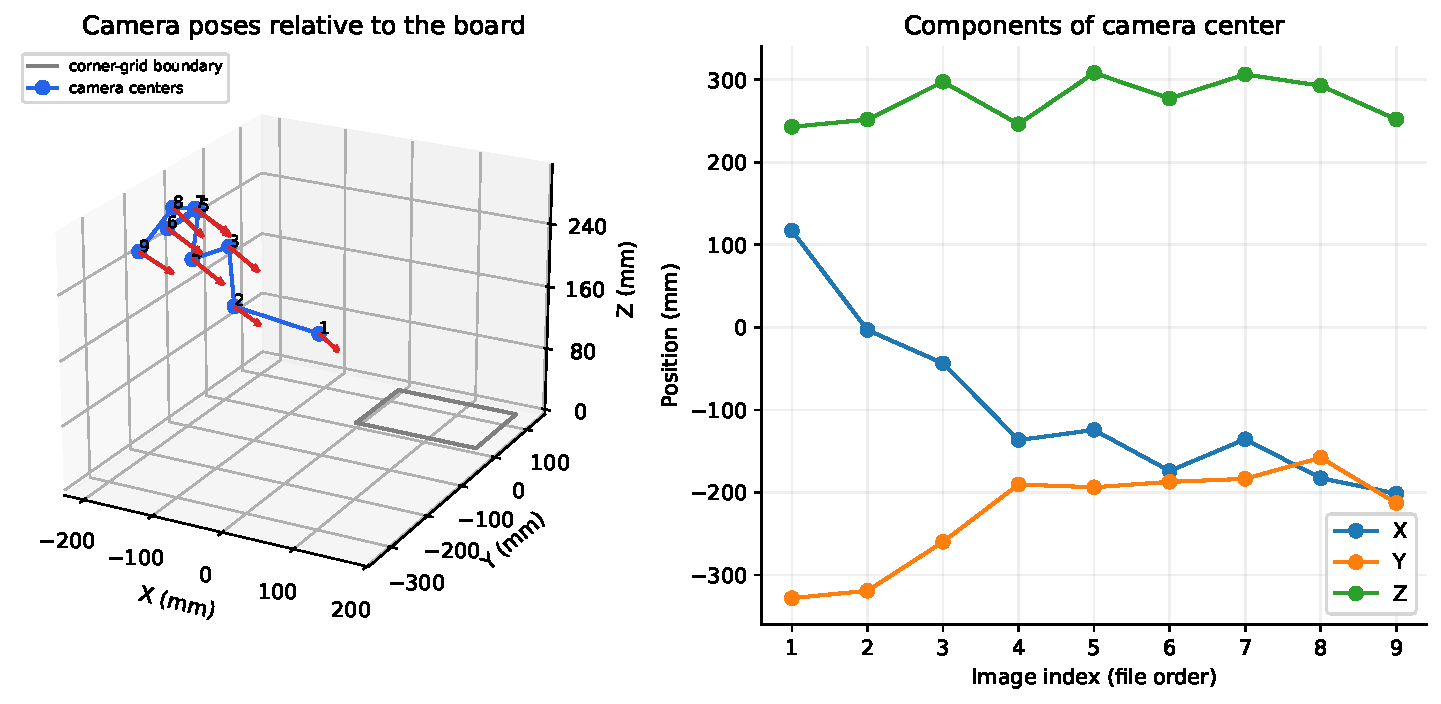
\includegraphics[width=\linewidth]{results/trajectory.pdf}
\caption{Recovered camera centers and optical directions in the checkerboard
frame (left), and coordinate values by view (right). Red arrows point along
each camera's forward optical axis, $R\T(0,0,1)\T$.}
\end{figure}
The camera lies on the positive-$Z$ side of the checkerboard, with recovered
board-normal distances between $242.880$ and $308.180$ mm. Its center moves
mainly toward decreasing $X$, with several reversals visible in the other
coordinates. The polyline joins the poses in file order; without timestamps,
it does not determine speed or a continuous motion path. These are camera
poses \emph{relative to the board}. Interpreting them as the camera's motion
in a fixed external world assumes the board stayed fixed.

\clearpage
\appendix
\section{Complete code used for the assignment}
\lstinputlisting[basicstyle=\ttfamily\fontsize{8}{9.2}\selectfont]{solve_hw1.py}
\end{document}
